\documentclass[11pt,a4paper]{article}

% Page Layout - 2 cm margins on left and right
\usepackage[a4paper, left=2cm, right=2cm, top=2.5cm, bottom=2.5cm]{geometry}
\setlength{\parindent}{0pt}

% Fonts (XeLaTeX-native, replaces inputenc/fontenc/lmodern)
\usepackage{fontspec}
\setmainfont{Latin Modern Roman}
\setmonofont{DejaVu Sans Mono}   % or JuliaMono for full Julia glyph coverage
\usepackage{microtype}

% Colors
\usepackage{xcolor}
\definecolor{juliapurple}{RGB}{145, 53, 156}
\definecolor{juliagreen}{RGB}{56, 152, 38}
\definecolor{juliared}{RGB}{203, 60, 51}
\definecolor{juliablue}{RGB}{64, 99, 216}
\definecolor{codebg}{RGB}{248, 249, 250}
\definecolor{codeframe}{RGB}{220, 224, 230}
\definecolor{commentgray}{RGB}{108, 117, 125}

% Math & Symbols
\usepackage{amsmath, amssymb, amsfonts}

% Code Listing Configuration for Julia (minted)
\usepackage{minted}
\usemintedstyle{friendly}   % pygments style; try "colorful", "tango", "friendly" etc.

\setminted{
    frame            = single,
    rulecolor        = \color{codeframe},
    framesep         = 6pt,
    bgcolor          = codebg,
    fontsize         = \small,
    breaklines       = true,
    breakafter       = ,        % allow breaks anywhere if needed; tune as desired
    linenos          = true,
    numbersep        = 10pt,
    tabsize          = 4,
    baselinestretch  = 1.0,
}

\setminted[julia]{
    % julia-specific overrides go here if you ever want them
}

% Hyperlinks
\usepackage{hyperref}
\hypersetup{
    colorlinks=true,
    linkcolor=juliablue,
    citecolor=juliagreen,
    urlcolor=juliapurple
}

% Figures
\usepackage{graphicx}
\usepackage{subcaption}

% Title Metadata
\title{\textbf{Simulations and Dynamics Course Report}\\ \large Numerical Integration \& Nonlinear Dynamical Systems}
\author{\textbf{Author Name} \\ Course Code: SD-401}
\date{\today}

\begin{document}

\maketitle

\begin{abstract}
This will contain an abstract at some point.
\end{abstract}

\section{Setting up Problems and ODEs for a Single Particle}

A simple pendulum with a point mass is taken as an exemplar point particle problem. The second order equation of motion is written as a system of first order ODEs in julia.

\begin{equation}
    \ddot{\theta} + \frac{g}{l} \sin\left(\theta\right)
\end{equation}

where $g$ is the acceleration due to gravity, $l$ is the length of the string of the point-mass pendulum and $\theta(t)$ is the angle that the string makes with the normal axis.

\begin{minted}{julia}
function system!(du, u, p, t)
    # Unpack state vector
    ϕ_1, ϕ_2 = u
    l, g = p

    # Define time differentials
    dϕ_1 = ϕ_2
    dϕ_2 = -g/l * sin(ϕ_1)

    du[1] = dϕ_1
    du[2] = dϕ_2
    return nothing
end
\end{minted}

\begin{figure}[htbp]
    \centering
    \begin{subfigure}[b]{0.48\textwidth}
        \centering
        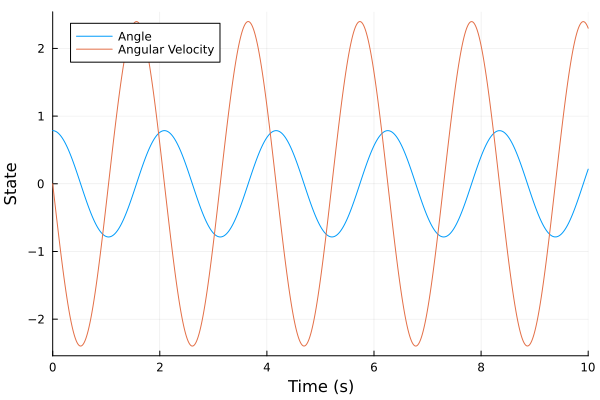
\includegraphics[width=\textwidth]{Problems/Problem1/figures/state_plot.png}
        \caption{Time-Dependent Solutions}
    \end{subfigure}
    \hfill
    \begin{subfigure}[b]{0.48\textwidth}
        \centering
        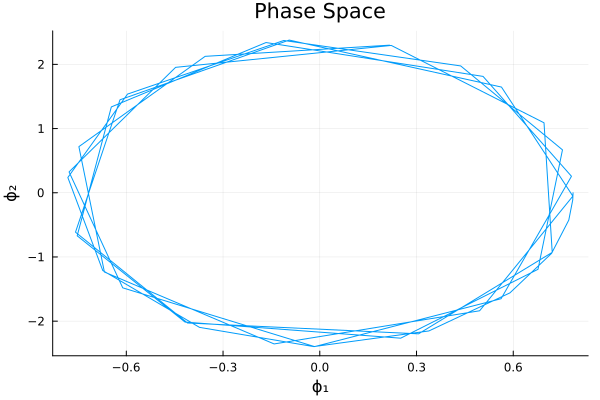
\includegraphics[width=\textwidth]{Problems/Problem1/figures/phase_space.png}
        \caption{Phase Space}
    \end{subfigure}
    \caption{Solution}
\end{figure}

The solution of the problem was animated.

\begin{minted}{julia}
animation = @animate for t in range(tspan[1], tspan[2], length = 200)
    θ = solution(t)[1]
    dθ = solution(t)[2] # We will not be using this result here

    x = l * sin(θ)
    y = -l * cos(θ)

    # Animate the string too!
    plot(
        [0, x],
        [0, y],
        lw = 3,
        color = :black,
        aspect_ratio =:equal,
        xlims=(-1.2l, 1.2l), ylims=(-1.2l, 0.2l)
    )

    # Animate the mass
    scatter!(
        [x], [y], color = :red, ms = 12
    )
end
\end{minted}
\section{Getting better with Vectors}
\subsection{The shortest distance between two lines}
Consider four points $A, B, C$ and $D$ described by vectors $\vec{r}_A, \vec{r}_B, \vec{r}_C, \vec{r}_D$.

The shortest distance between two lines can be represented by the line segment that intersects both lines perpendicularly. We thus define two vectors that go through $\vec{r}_A$ and $\vec{r}_B$, and $\vec{r}_C$ and $\vec{r}_D$, with directions

$$
\vec{u} = \vec{r}_B - \vec{r}_A \\
\vec{v} = \vec{r}_D - \vec{r}_C.
$$

A mutually perpendicular direction is identified using the cross product of these two directions

$$
\vec{n} = \vec{u} \times \vec{v}
$$

which we turn into a unit vector by dividing it by its magnitude.

\begin{equation}
    \hat{n} = \frac{\vec{u} \times \vec{v}}{|| \vec{u} \times \vec{v} ||}
\end{equation}

Two planes containing each of the lines are constructed, while constraint to being parallel to the other line (the line that is not contained within the plane). Since both the planes are parallel to the other lines, the vector $\vec{n}$ is the normal vector to both planes.

To find the gap between these two planes, any point on the planes are chosen -- for example $\vec{r}_A$ and $\vec{r}_C$. A new vector $\vec{w} = \vec{r}_C - \vec{r}_A$ is drawn to connect them. To find the true distance between the two planes, the connecting vector is projected onto the perpendicular vector $\vec{n}$. Thus,

\begin{equation}
    d = |\vec{w} \cdot \vec{n}|.
\end{equation}

\subsection{Fixed Structure Problem}
Assume that points $A, B$ and $C$ are fixed to a structure, and all three are connected by massless rods to a ball and socket joint at each end, to point $D$. At point $D$ a force $\vec{F}$ is applied. In this section we attempt to find the tension in bar $AD$.

Let the tension vectors in rods $AD$, $BD$, and $CD$ be $\vec{T}_1 = T_1 \hat\lambda_1$, $\vec{T}_2 = T_2 \hat\lambda_2$ and $\vec{T}_3 = T_3 \hat\lambda_3$ respectively. We may then write the equation

\begin{equation}
    T_1 \lambda_1 + T_2 \lambda_2 + T_3 \lambda_3 = \vec{F}
\end{equation}

A vector normal to the unit direction vectors $\hat\lambda_2$ and $\hat\lambda_3$ is constructed

\begin{equation}
    \vec{n} = \hat\lambda
\end{equation}

and the force balance equation is projected onto the vector along $\vec{n}$. Since, by definition, $\vec{n} \perp \hat\lambda_2, \hat\lambda_3$,

\begin{equation}
    T_1 \left(\vec{n} \cdot \hat\lambda_1 \right) = \vec{n} \cdot \vec{F}
\end{equation}

and therefore,

\begin{equation}
    T_1 = \frac{\left(\vec{n} \cdot \vec{F}\right)}{\left(\vec{n} \cdot \hat\lambda_2\right)}.
\end{equation}


\section{ODE and Animation Practice}

The Lorentz System is chosen for this problem.

\begin{minted}{julia}
# Define a Lorentz System
function Lorentz_system!(du, u, p, t)
    # Unpack the system
    x, y, z = u
    σ, ρ, β = p

    # Dynamics
    dx = σ*(y - x)
    dy = x*(ρ - z) - y
    dz = x*y - β*z

    du[1] = dx; du[2] = dy; du[3] = dz
    return nothing # Absolutely nothing at all!
end
\end{minted}

\subsection{Implementation of Euler's Method}
An implementation of Euler's Method for solving ODEs is developed. This is defined as a single module as shown here.

\begin{minted}{julia}
module MySolvers

export ODESolution, Euler, euler_step!

# Define the solution data struct
struct ODESolution
    t::Vector{Float64}
    u::Vector{Vector{Float64}}
end

# Step wrapper (to prevent overpopulating the heap memory)
function euler_step!(system!, u, p, t, dt, du)
    system!(du, u, p, t)
    u .+= dt .* du
    return u
end

function Euler(
    system,
    initial_state::Vector{Float64},
    tspan::Tuple{Float64, Float64},
    parameters::Vector{Float64},
    delta_t::Float64
)
    t_start, t_stop = tspan
    number_of_steps = round(Int, (t_stop - t_start) / delta_t)

    t_vec = Vector{Float64}(undef, number_of_steps + 1)
    u_vec = Vector{Vector{Float64}}(undef, number_of_steps + 1)

    u_curr = copy(initial_state)
    du = similar(initial_state)
    t_curr = t_start

    t_vec[1] = t_curr
    u_vec[1] = copy(u_curr)

    for i in 1:number_of_steps
        euler_step!(system, u_curr, parameters, t_curr, delta_t, du)
        t_curr += delta_t

        t_vec[i + 1] = t_curr
        u_vec[i + 1] = copy(u_curr)
    end

    return ODESolution(t_vec, u_vec)
end
end # module
\end{minted}

\begin{figure}
    \centering
    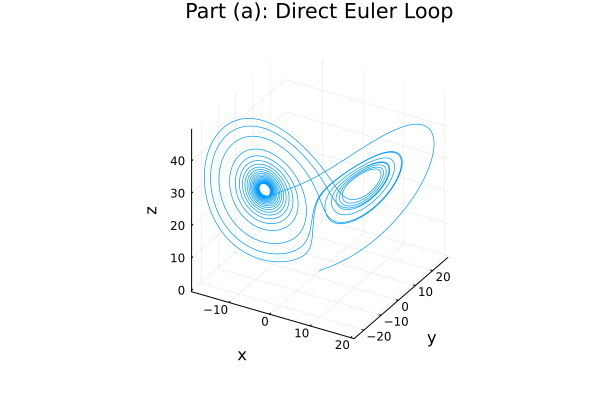
\includegraphics[width = 0.8 \textwidth]{Problems/Problem3/figures/lorenz_direct.png}
    \caption{Solution of the System using Euler's Method}
\end{figure}

\subsection{Estimating Accuracy}
One of the methods one can use to determine the accurracy of this implementation of Euler's Method is to compare its results to that of a higher order solver. For this purpose, the eigth-order solver \texttt{Vern8()} is used, with absolute and relative tolerances of $10^{-13}$.

In order to observe the change in accuracy of Euler's method, the time internal between consecutive integrations $dt$ is varied.

\begin{figure}
    \centering
    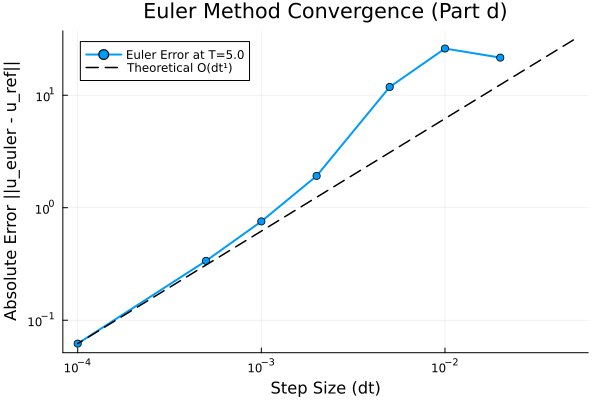
\includegraphics[width = 0.8 \textwidth]{Problems/Problem3/figures/euler_convergence.png}
\end{figure}

\subsubsection{Estimating Accuracy without Absolute References}
As shown in my Robotic Motion and Simulation report, one can estimate the accuracy of one's results using the Euler Method without an exact solution or high precision solver.


Estimating errors in numerical ODE solving (Euler's Method) and the relation so step size. This can be done without knowing the exact analytical solution. We know that

\begin{equation}
    x_{t+1}^{(h)} = x_t + h f(x_t, t),
\end{equation}

and thus

\begin{equation}
    x_{t+1}^{(h/2)} = x_t + \frac{h}{2} f(x_t, t).
\end{equation}

If we define the exact solution of the ODE to be $y_t$, and assuming that the error in Euler's Method is $\mathcal{O}(h)$, we may write that

\begin{equation}
    y_t = x_t^{(h)} + Ch + \mathcal{O}(h^2).
\end{equation}

With the difference

\begin{equation}
    x_t^{(h/2)} - x_t^{(h)} = \bigg(y_t - C\frac{h}{2} - \mathcal{O}(h^2)\bigg) - \bigg(y_t - Ch - \mathcal{O}(h^2)\bigg)
\end{equation}

and ignoring the $\mathcal{O}(h^2)$ term,

\begin{equation}
    x_t^{(h)} - x_t^{(h/2)} = C \frac{h}{2}.
\end{equation}

Thus, we may estimate the error $Ch = y_t - x_t^{(h)}$ as

\begin{equation}
    \text{error}(h) \approx 2 \bigg(x_t^{(h)} - x_t^{(h/2)} \bigg)
\end{equation}

\subsection{5thb Order Solvers (RK45)}
For a more pratical approach to numerically solving systems such as these, one may utilize 5th order solvers such as \texttt{RK45} or \texttt{Tsit5}.

\begin{figure}
    \centering
    \begin{subfigure}[b]{0.48\textwidth}
        \centering
        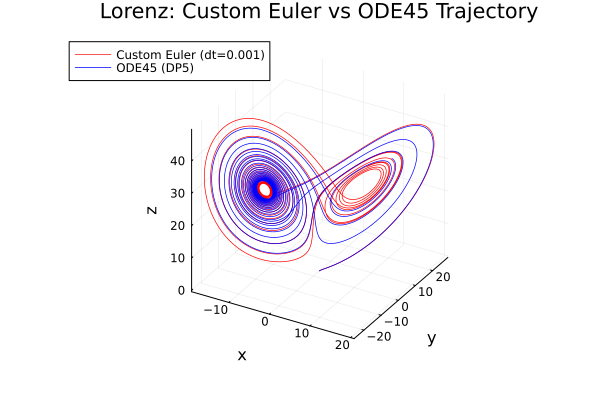
\includegraphics[width=\textwidth]{Problems/Problem3/figures/comparison_euler_vs_ode45_3d.png}
        \caption{Trajectory Comparision -- Euler's Method vs Tsit5}
    \end{subfigure}
    \hfill
    \begin{subfigure}[b]{0.48\textwidth}
        \centering
        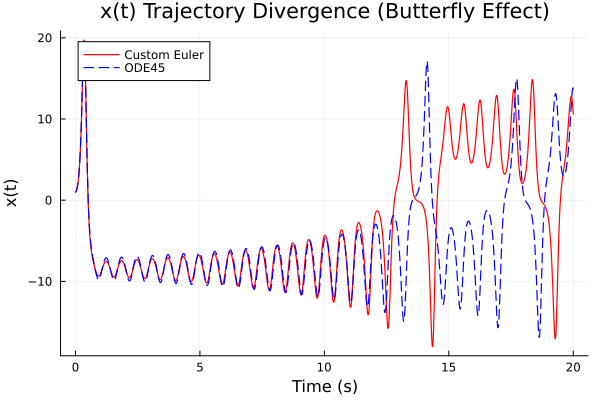
\includegraphics[width=\textwidth]{Problems/Problem3/figures/comparison_euler_vs_ode45_time.png}
        \caption{Trajectory Divergence -- -- Euler's Method vs Tsit5}
    \end{subfigure}
    \caption{5th Order Solution Results and Comparisons}
\end{figure}

\subsection{Error Estimation -- 5th Order Solvers}
A low-tolerance 8th order solver is used as a reference to compare \texttt{Tsit5} results to.

\begin{figure}
    \centering
    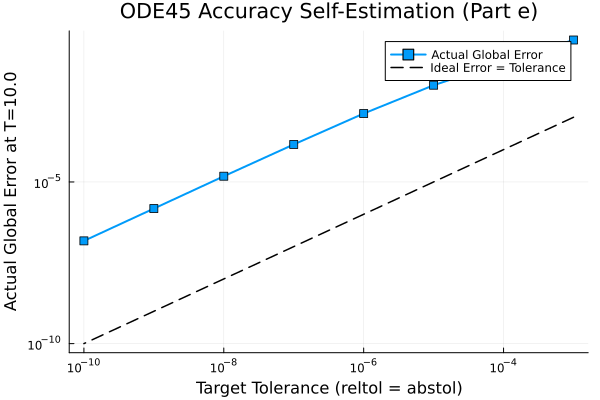
\includegraphics[width = 0.8 \textwidth]{Problems/Problem3/figures/ode45_accuracy_assessment.png}
\end{figure}

\begin{minted}{julia}
target_tols = 10.0 .^ (-3:-1:-10)
actual_errors = Float64[]

# High-precision ground truth at T = 10.0
T_tol_eval = 10.0
u_true_T = sol_ref(T_tol_eval)

for tol in target_tols
    sol_tol = solve(prob, DP5(), reltol=tol, abstol=tol)
    u_final_tol = sol_tol(T_tol_eval)
    push!(actual_errors, norm(u_final_tol - u_true_T))
end

# Tolerance Assessment Plot
plt_tol = plot(target_tols, actual_errors, xscale=:log10, yscale=:log10,
               marker=:square, lw=2, label="Actual Global Error",
               xlabel="Target Tolerance (reltol = abstol)", 
               ylabel="Actual Global Error at T=10.0",
               title="ODE45 Accuracy Self-Estimation (Part e)")

plot!(plt_tol, target_tols, target_tols, label="Ideal Error = Tolerance", 
      ls=:dash, color=:black, lw=1.5)
\end{minted}

Julia's \texttt{Tsit5()} solver does not (seem to) appear self-error estimation. This claim must be investigated.

\end{document}